
\section{Lecture 5 - 26.01.21}

We will first prove the theorem we left off at last time. We recall its statement.

\begin{theorem}
Let $F, G\in K[X, Y]$ be two non-zero polynomials with no common factors. Then $V(F)\cap V(G)$ is finite. 
\end{theorem}
\begin{proof}
Let $(x, y)\in V(F)\cap V(G)$. This means in particular that $F(x, y)=0=G(x, y)$. By the lemma we proved last time there exists some $d\in k[X]$ such that $d=AF+BG$. Since both $F$ and $G$ vanish on $(x, y)$ we have $d(x)=0$. Since $d$ is a polynomial in one variable over a field it has only a finite set of roots. Hence we only have finite choices for $x$. 

Symmetrically we can find a polynomial $d'\in k[Y]$ with the same above properties. By the same argument er only have finite choices for $y$. Hence $V(F)\cap V(G)$ is a finite set. 
\end{proof}

\begin{theorem}
Let $F, G\in K[X, Y]$ be two non-zero polynomials with no common factors. Then $k[X, Y]/(F, G)$ is a finite dimensional vector space. 
\end{theorem}
\begin{problem}
Compare this to \cref{prop:finite_iff_fin-dim-vs}
\end{problem}
\begin{proof}
By the same lemma used before we know there exists $d, d'\in (F, G)$ such that $d\in k[X]$ and $d'\in k[Y]$. Write
\begin{itemize}
    \item $d(X)=X^n+a_{n-1}X^{n-1}+\ldots +a_0$
    \item $d'(Y)=Y^m+b_{m-1}Y^{m-1}+\ldots +b_0$
\end{itemize}
There are both zero in $k[X, Y]/(F, G)$ as they belong to $(F, G)$. Hence, in $k[X, Y]/(F, G)$ we have $X^n\in (X^{n-1}, \ldots, X, 1)$ and $Y^m\in (Y^{m-1}, \ldots, Y, 1)$, which means
\begin{equation*}
    \{ X^i Y^j \}_{0\leq i\leq n-1, 0\leq j\leq m-1}
\end{equation*}
is a generating set for $k[X, Y]/(F, G)$. This set is finite, which means we are done we are done. 
\end{proof}

\begin{example}
Find a generating set for $k[X, Y]/(X^3, Y^2-X)$.
\end{example}
We can think of the generators as the following system. 
\begin{center}
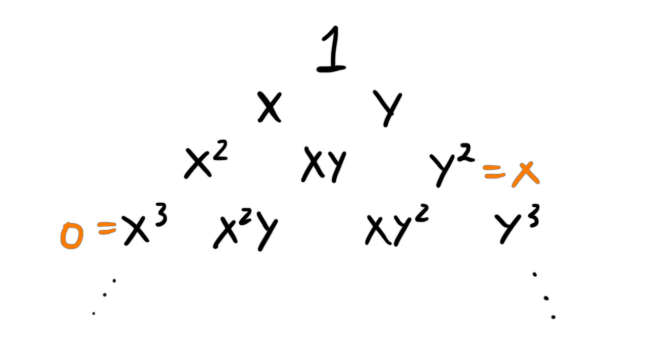
\includegraphics[width=8cm]{img/lecture_5/system1.png}
\end{center}
The relations makes some products of generators die. If we continue this we get something like:
\begin{center}
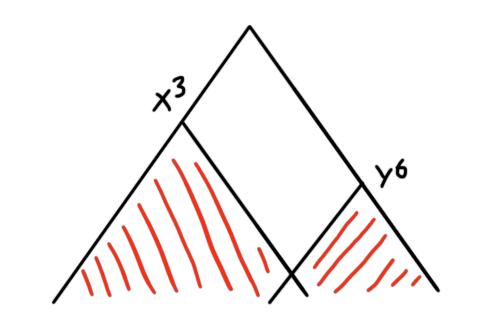
\includegraphics[width=8cm]{img/lecture_5/system2.png}
\end{center}
And we can then count the ones that have not perished (the ones inside the non-red area). 

\subsection{Introduction to morphisms}

For this part we let $k$ be an infinite field. 

\begin{definition}[Regular map]
Let $V\subset k^n$, $W\subset k^m$ be affine algebraic sets. A morphism, called a regular map, $\phi:V\longrightarrow W$ is a collection of maps $\phi_i:k^n\longrightarrow k^m$ such that each $\phi_i$ is polynomial, i.e. $\phi_i\in\Gamma(V)$. 
\end{definition}

We denote the set of regular maps between $V$ and $W$ by $Reg(V, W)$. These maps make the collection of affine algebraic sets over $k$ into a category, denoted $Aff(k)$. 

\begin{remark}
The regular maps are continuous in the Zariski topology, but they are not all of the continuous maps. 
\end{remark}

\begin{example}
Elements of $\Gamma(V)$ are the regular maps $V\longrightarrow k$.
\end{example}

\begin{example}
Any projection $V\subset k^n\longrightarrow k^p$, where $p\leq n$ is a regular map. 
\end{example}

\begin{example}
$\phi: V(Y-X^2)\longrightarrow k$ defined by $(x, y)\mapsto x$ is actually a regular isomorphism. The inverse is given by $\phi^{-1}(x)=(x, x^2)$. Visually it looks like

\begin{center}
\def\svgwidth{0.4\textwidth}
\input{inkscape/parable_regular_isomorphism.pdf_tex}
\end{center}
\end{example}


\begin{example}
$\phi:V(X^2+Y^2-1)$ sending $(x, y)\mapsto x$ is regular but not injective. It looks like

\begin{center}
\def\svgwidth{0.4\textwidth}
\input{inkscape/circle_regular_morphism.pdf_tex}
\end{center}
\end{example}


Let $\phi:V\longrightarrow W$ be regular map. For any $f\in \Gamma(W)$ we set $\phi^*(f)=f\circ\phi \in \Gamma(V)$, i.e. the pre-composition with $\phi$. This makes $\Gamma$ into a contravariant functor. It sends $V$ to $\Gamma(V)$ and $\phi:V\longrightarrow W$ to $\phi^*:\Gamma(W)\longrightarrow \Gamma(V)$. 

\begin{proposition}
The functor $\Gamma$ is a fully faithful functor. 
\end{proposition}

We can in fact show something even stronger. 

\begin{theorem}
Let $k$ be algebraically closed, and let $ftr-Alg_k$ denote the category of finite type reduced $k$-algebras. Then we have an equivalence of categories
\begin{equation*}
    \Gamma: Aff(k)\longrightarrow ftr-Alg_k
\end{equation*}
\end{theorem}
Before we prove this lets justify that $\Gamma$ only hits these types of algebras. We know that $\Gamma(V)\cong k[X_1, \ldots, X_n]/I(V)$ is a $k$-algebra, and it is generated by $x_1, \ldots, x_n$ and is thus of finite type. Such a $k$-algebra is reduced if and only if $I(V)$ is a radical ideal. This we know is true by Hilbert's nullstellensatz, hence we know that algebras in the image of $\Gamma$ are in $ftr-Alg_k$. 

\begin{proof}
Lets first show that $\Gamma$ is fully faithful. This means that it is an isomorphism on the sets of morphisms. We start with showing it is injective. 

Let $\phi, \psi\colon V\longrightarrow W$ be regular maps such that $\phi^*=\psi^*$. Through the isomorphisms $\Gamma(W)\cong k[Y_1, \ldots, Y_m]/I(W)$ and $\Gamma(V)\cong k[X_1, \ldots,X_n]/I(V)$ we have that $\phi^*$ sends $Y_i$ to $\phi_i$. Since $\psi^*$ also does this they must have the same images, i.e. $\phi_i = \psi_i$. Since all the components are the same the maps are the same. 

We now show $\Gamma$ is surjective on the morphisms. 

Let $\theta:k[Y_1, \ldots, Y_m]/I(W) \longrightarrow k[X_1, \ldots,X_n]/I(V)$ be an algebra morphism. Set $\phi_i = \theta(Y_i)$ and $\phi = (\phi_1, \ldots, \phi_m)$. We claim that $\phi:V\longrightarrow W$, i.e. $\Ima \phi \subseteq W$ and hence that $\Gamma$ is surjective on morphisms. 

For $\Gamma$ to be an equivalence of categories we also need it to be a dense functor, also called essentially surjective. 

Let $A$ be a finite type reduced $k$-algebra. Since $A$ is of finite type we have some generators $X_1, \ldots, X_n$ and some relations, that generate an ideal $I$, such that $A=k[X_1, \ldots, X_n]/I$. Since $A$ is reduced wee know that $I$ is a radical ideal. By Hilbert's nullstellensatz we know that $I=I(V(I))$, and hence we have $A\cong \Gamma(V(I))$.

This shows that $\Gamma$ is an equivalence of categories. 
\end{proof}
\todo[inline]{Show surjectivity}


\subsection{Projective algebraic sets}

Affine algebraic sets are nice and easy, but they have some problem. Most notably for us now is the case of intersection points of curves. The general structure is that two lines always meet at a point, but this has an exception, namely parallel curves. 

\begin{center}
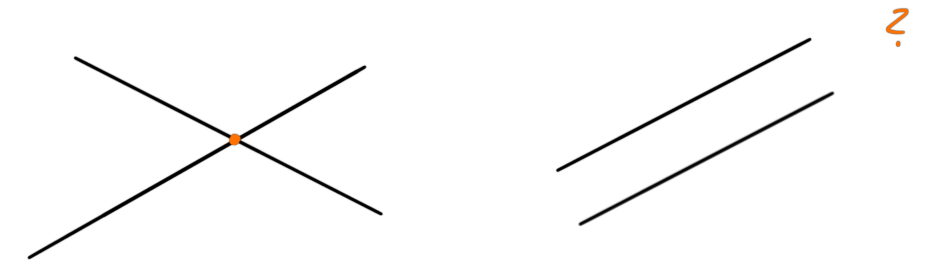
\includegraphics[width=12cm]{img/lecture_5/projective1.png}
\end{center}

The reason we move to projective algebraic sets instead is that these exceptions disappear. 


\begin{definition}
Let $n\geq 0$ be an integer and let $E$ be a $k$-vector space of dimension $n+1$. For $x, y\in E\setminus\{0\}$ we define the relation $x\sim y$ if there exists a $\lambda \in k^\times$ such that $y=\lambda x$. 
\end{definition}

\begin{problem}
Show that this relation is an equivalence relation.
\end{problem}

Note that the equivalence classes of this relations are the lines in $E$ through the origin. 

\begin{definition}[Projective space]
The projective space of $E$, denoted $\P(E)$, is the set $(E\setminus \{0\})/\sim$, i.e. the set of lines in $E$. 
\end{definition}

If $E=k^n$ then $\P(E)=\P^n(k)$ is called the standard projective $n$-space \index{Standard projective space}.

Let $\pi:k^{n+1}\setminus \{0\}\longrightarrow \P^n(k)$ be the canonical projection, and let $x=(x_0, \ldots, x_n)\in k^n\setminus\{0\}$. Then $\bar{x}=\pi(x)$ is a point in $\P^n(k)$ with homogeneous coordinates $(x_0, \ldots, x_n)$ often written $[x_0:\cdots :x_n]$. 

Note that if $\lambda\neq 0$, then $[\lambda x_0:\cdots :\lambda x_n]$ is another system of homogeneous coordinates for $\bar{x}$. 

\begin{example}
Let $k=\R$. Then $\P^1(\R)$ is the set of lines trough the origin in $\R^2$. 
\end{example}

\begin{problem}
Read and learn about projective space. 
\end{problem}
\label{lec5:visualization}


\iffalse
\begin{solution}

One way to understand projective $1$-space is the following. We can think about $k^2$ using the standard plane with basis $x, y$. We can then think about $\P^1(k)$ as a line through $y=1$. 

\begin{center}
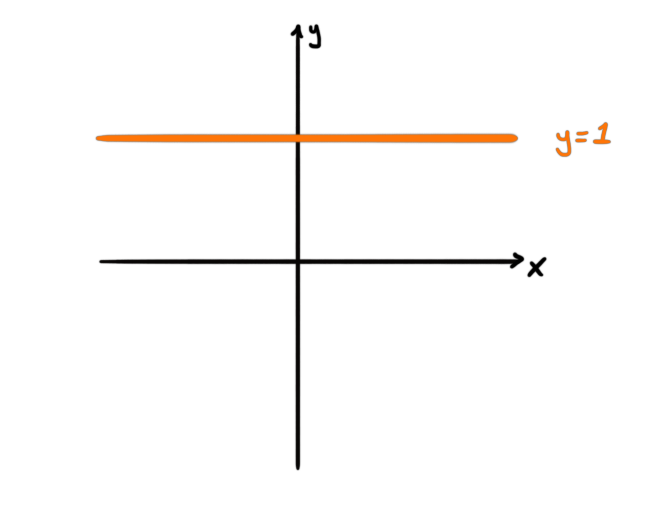
\includegraphics[width=8cm]{img/lecture_5/projective2.png}
\end{center}

Every line through the origin in $k^2$ now corresponds to a point on $\P^1(k)$. 

\begin{center}
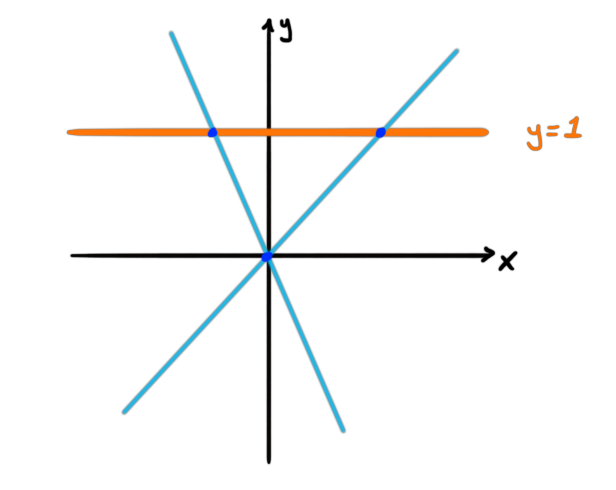
\includegraphics[width=8cm]{img/lecture_5/projective3.png}
\end{center}

But we also have one unique line that does not pass through $\P^1(k)$, namely the line $y=0$. We think of this line as intersecting $\P^1(k)$ at infinity. 

\begin{center}
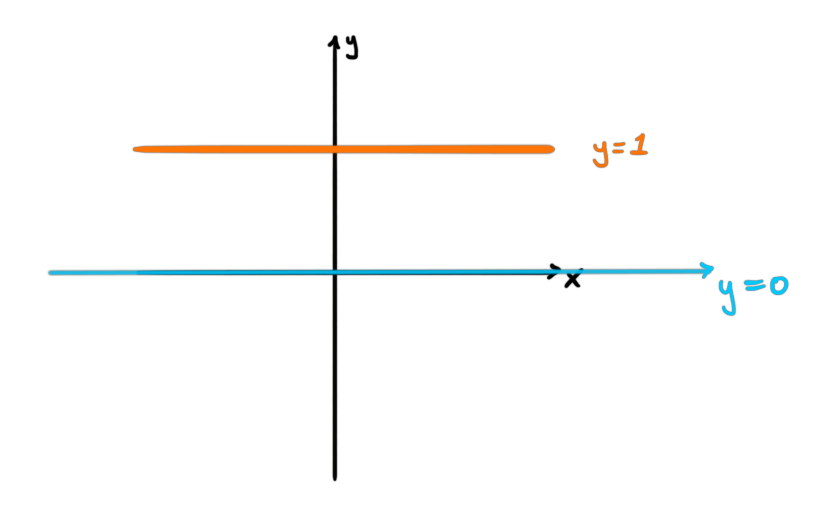
\includegraphics[width=8cm]{img/lecture_5/projective4.png}
\end{center}

This becomes even better when we pass to $\P^2(k)$ which are the set of lines through $k^3$. We still set $\P^2(k)$ as the now plane $z=1$. 

\begin{center}
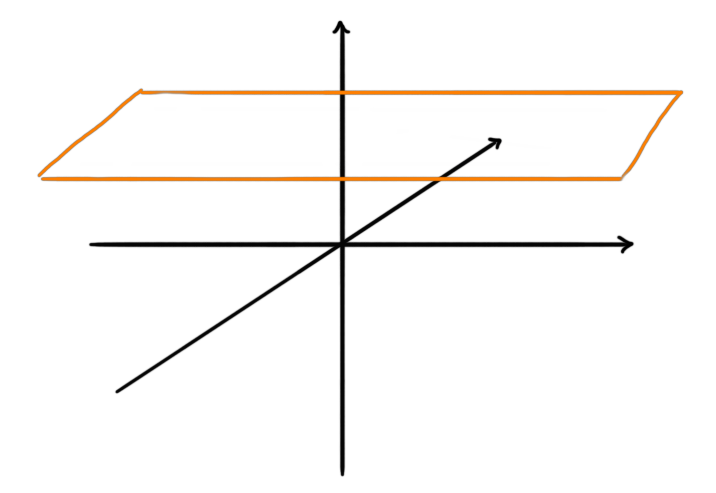
\includegraphics[width=8cm]{img/lecture_5/projective4.5.png}
\end{center}

We still have that any line through the origin uniquely describes a point on $\P^2(k)$. 
\begin{center}
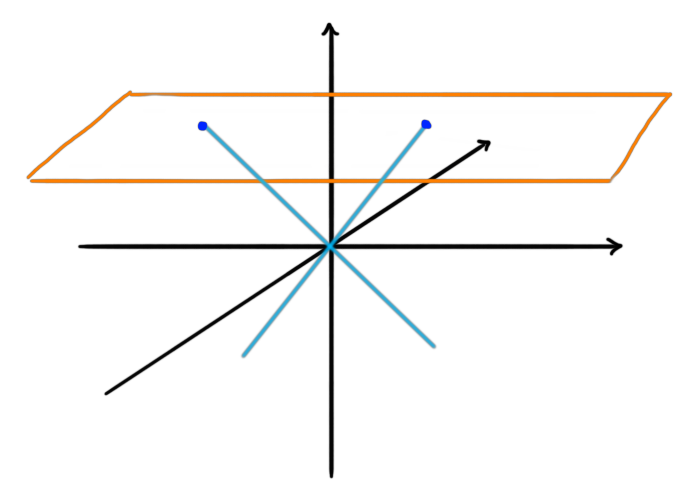
\includegraphics[width=8cm]{img/lecture_5/projective4.6.png}
\end{center}

But not we can discuss lines in $\P^2(k)$ as well! Notice a line corresponds exactly to a plane passing through the origin. If we now have two line we get a line from their intersection. This line will be a line through the origin, and it will meet $\P^2(k)$ exactly at the intersection of the two lines.
\begin{center}
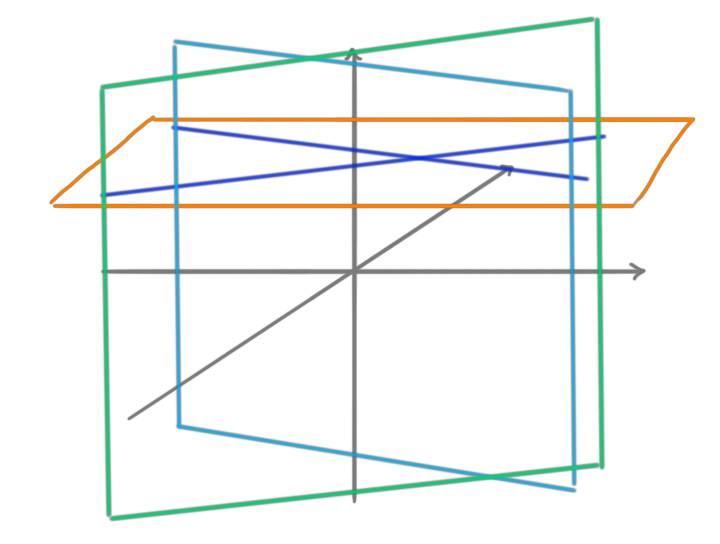
\includegraphics[width=8cm]{img/lecture_5/projective5.png}
\end{center}

But now even parallel lines meet at a line in the $XY$-plane, which we as earlier can think of as meeting $\P^2(k)$ at infinity. 

\begin{center}
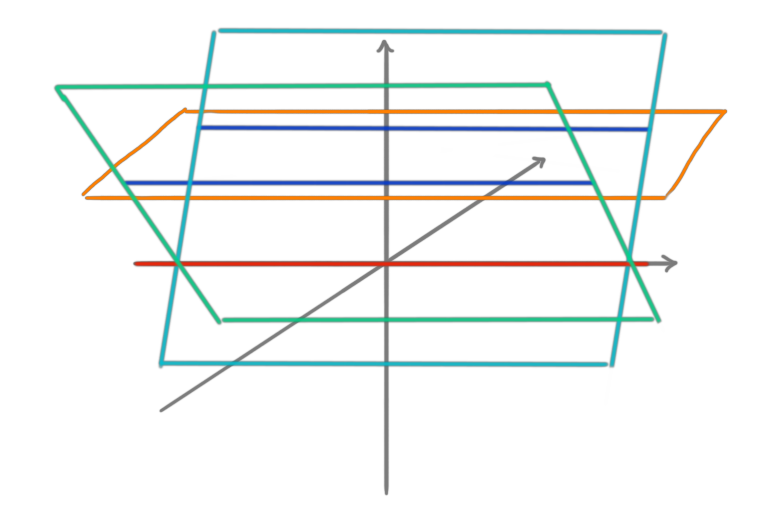
\includegraphics[width=8cm]{img/lecture_5/projective6.png}
\end{center}

Now all lines meet at a point, which is what we want! This is not a rigorous treatment, and we will cover this more mathematically in class. 

\end{solution}

\fi